\documentclass{beamer}
\usepackage{amsmath}
\usepackage{svg}
\usepackage{graphics}
\usepackage{bm}
\usetheme{metropolis}
\title{Stiff Set (1)}
\date{\today}
\author{Yunwen Chen,Yangjie Xu,Meng Su,Dandan Che,Zhengqiang Li,Xiaoyan Liu}
\institute{Shenzhen Institute of Advanced Technology,Chinese Academy of Sciences}
\begin{document}
\maketitle
\begin{frame}{Overview}
    \tableofcontents
\end{frame}
 \section{Problem}


 %\begin{frame}{Stiff set}
 %      $$ u_t^' = 98u+198v $$
 %       $$ v_t^' = -99u+-199v$$
 %\end{frame}
 \begin{frame}{Stiff Set}
    
    \[
        \begin{cases}
        u_t^{'} &= 98u+198v\\
        v_t^{'} &= -99u-199v
        \end{cases}
    \]

    $$u(0)=1,v(0)=1$$
    $$0\leq t \leq T =100$$.

 \end{frame}

 \begin{frame}{Exact Solution}
    \[
        \begin{cases}
        u(t) &= -3e^{-100t}+4e^{-t}\\
        v(t) &= 3e^{-100t}-2e^{-t}
        \end{cases}
    \]
    \end{frame}

\begin{frame}{How to evaluate numerical solution ?}
    For a vector $\bm{x}$,we define the norm
    $$||\bm{x}||= max |\bm{x}_i|$$
    consequently,we can evaluate the numerical solution by using
    $$||\bm{u}-\bm{u}_l||$$
    where $\bm{u}_l$ is the numerical solution  and $\bm{u}$ is exact solution at the numerical solution points.

\end{frame} 


 \section{Explicit Euler Method}
 \begin{frame}{Explicit Euler Method}
    Explicit Euler method for this problem
    \[
        \begin{cases}
        \frac{u_{n+1}-u_n}{h} &= 98u_n+198v_n\\
        \frac{v_{n+1}-v_n}{h} &= -99v_n-199v_n
        \end{cases}
    \]
    it can be presented as 
    \[
        \begin{cases}
        u_{n+1} &= (98u_n+198v_n)h+u_n\\
        v_{n+1} &= (-99u_n-199v_n)h+v_n
        \end{cases}
    \]
    \end{frame}

 \begin{frame}{Explicit Euler Result of $u(t)$}
    \centering
    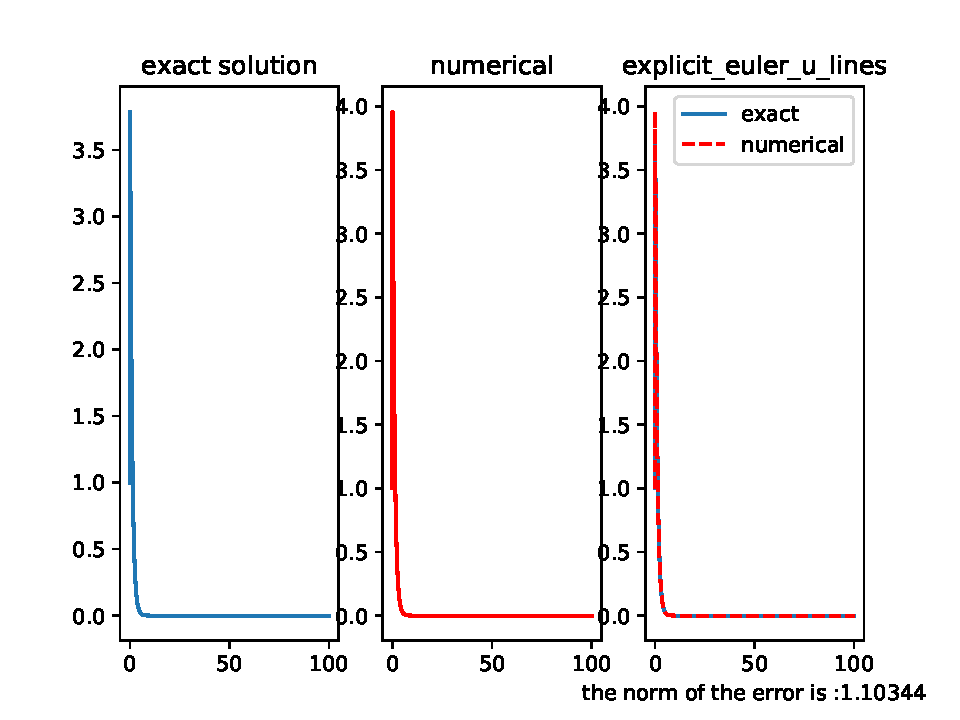
\includegraphics[height=8cm,width=12cm]{explicit_euler_u_lines.pdf}
 \end{frame}

 \begin{frame}{Explicit Euler Result of $v(t)$}
    \centering
    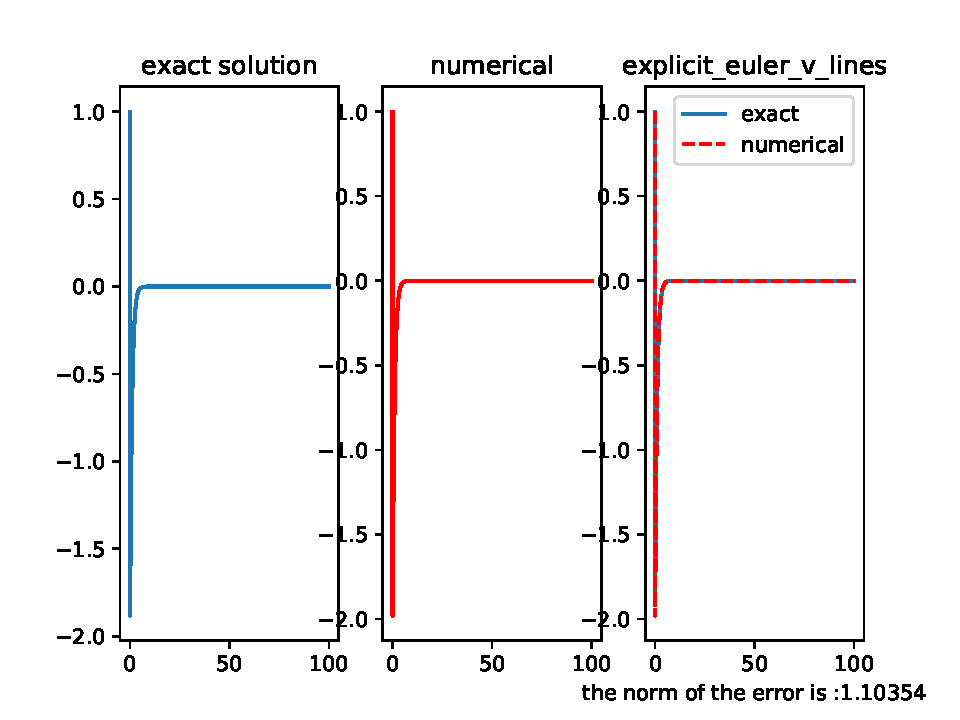
\includegraphics[height=8cm,width=12cm]{explicit_euler_v_lines.pdf}
 \end{frame}

 

 \section{Implicit Euler Method}
 \begin{frame}{Implicit Euler Method}
    Implicit Euler method for this problem
    \[
        \begin{cases}
        \frac{u_{n+1}-u_n}{h} &= 98u_{n+1}+198v_{n+1}\\
        \frac{v_{n+1}-v_n}{h} &= -99u_{n+1}-199v_{n+1}
        \end{cases}
    \]
    it can be presented as 
    \[
        \begin{cases}
        u_{n+1} &= \frac{(1+199h)u_n+198 h v_n}{(1-98h)(1+199h)+(198h)(99h)}\\
        v_{n+1} &= \frac{-99hu_n+(1-98h)v_n}{(1-98h)(1+199h)+(198h)(99h)}
        \end{cases}
    \]
    \end{frame}

 \begin{frame}{Implicit Euler Result of $u(t)$}
    \centering
    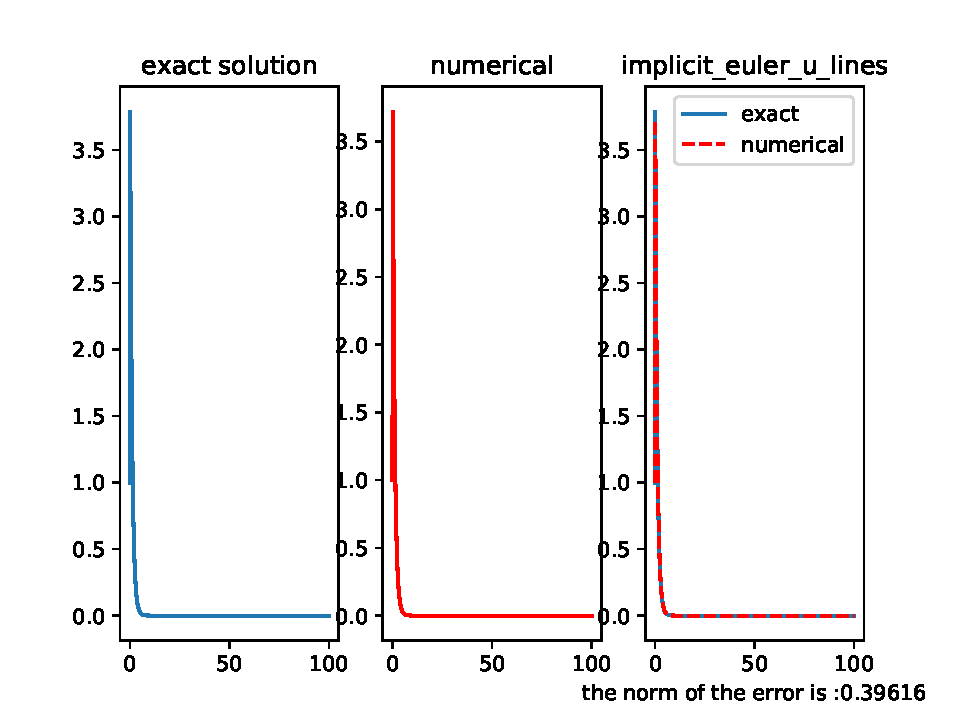
\includegraphics[height=8cm,width=12cm]{implicit_euler_u_lines.pdf}
 \end{frame}
 \begin{frame}{Implicit Euler Result of $v(t)$}
    \centering
    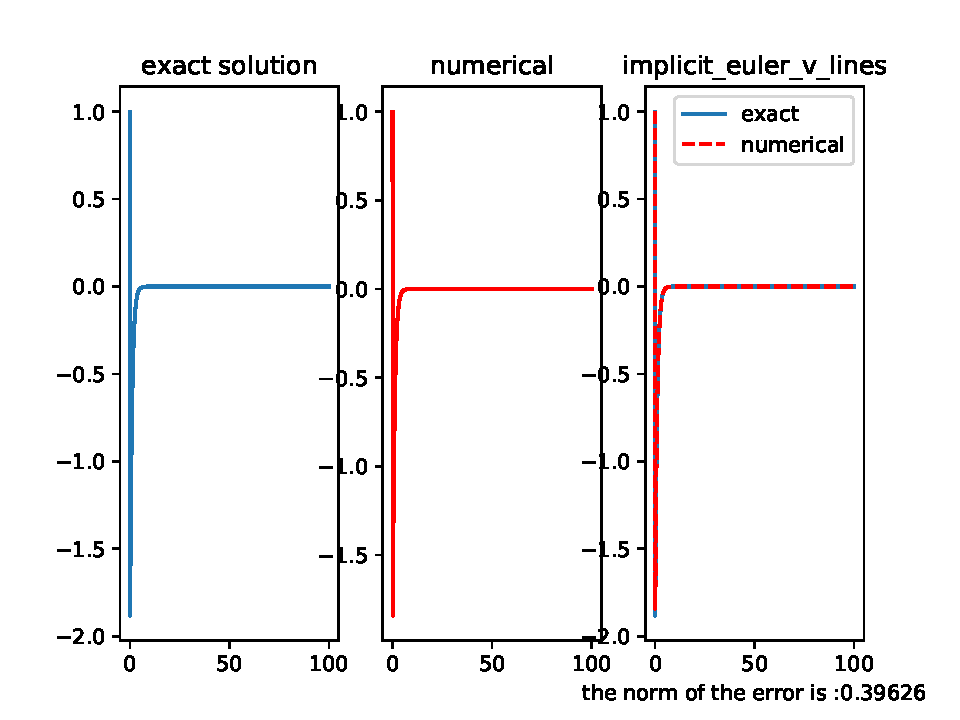
\includegraphics[height=8cm,width=12cm]{implicit_euler_v_lines.pdf}
 \end{frame}




 \section{Implicit Midpoint Method}
   \begin{frame}{Implicit Midpoint Method}
    Implicit midpoint method for this problem
    \[
        \begin{cases}
        \frac{u_{n+1}-u_n}{h} &= 98\frac{u_n+u_{n+1}}{2}+198\frac{v_n+v_{n+1}}{2}\\
        \frac{v_{n+1}-v_n}{h} &= -99\frac{u_n+u_{n+1}}{2}-199\frac{v_n+v_{n+1}}{2}
        \end{cases}
    \]
    We use the iterator method to obtain the numerical solution
    \[
        \begin{cases}
        u_{n+1}^{(s+1)} &= 98h\frac{u_n+u_{n+1}^{(s)}}{2}+198h\frac{v_n+v_{n+1}^{(s)}}{2}+u_n\\
        v_{n+1}^(s+1) &= -99h\frac{v_n+v_{n+1}^{(s)}}{2}-199h\frac{v_n+v_{n+1}^{(s)}}{2}+v_n
        \end{cases}
        \]
    \end{frame}
 \begin{frame}{Implicit Midpoint Result of $u(t)$}
    \centering
    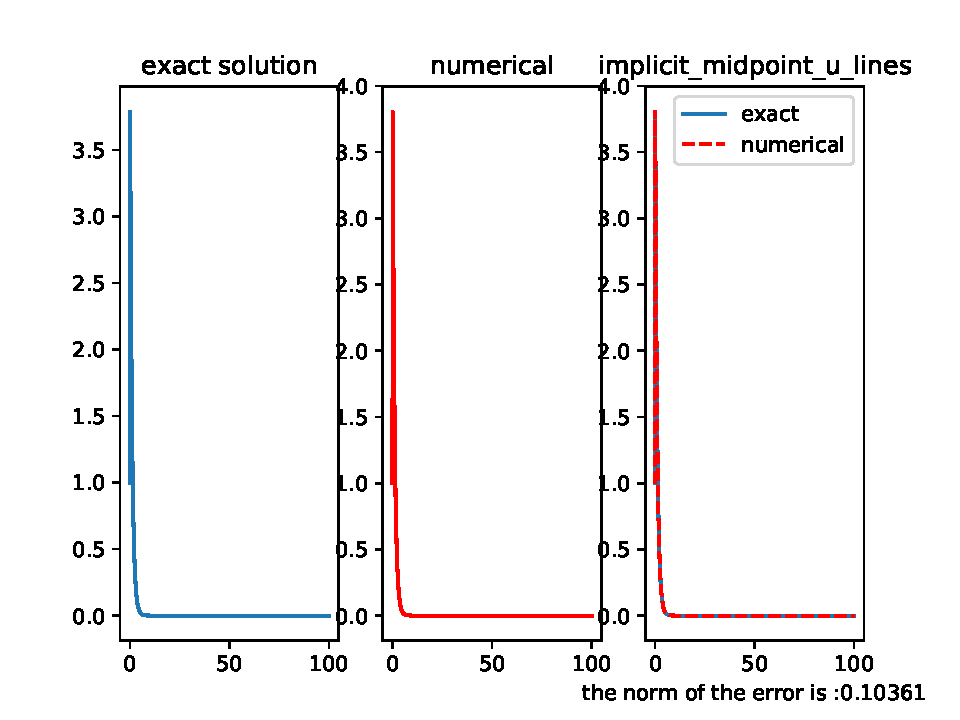
\includegraphics[height=8cm,width=12cm]{implicit_midpoint_u_lines.pdf}
 \end{frame}
 \begin{frame}{Implicit Midpoint Result of $v(t)$}
    \centering
    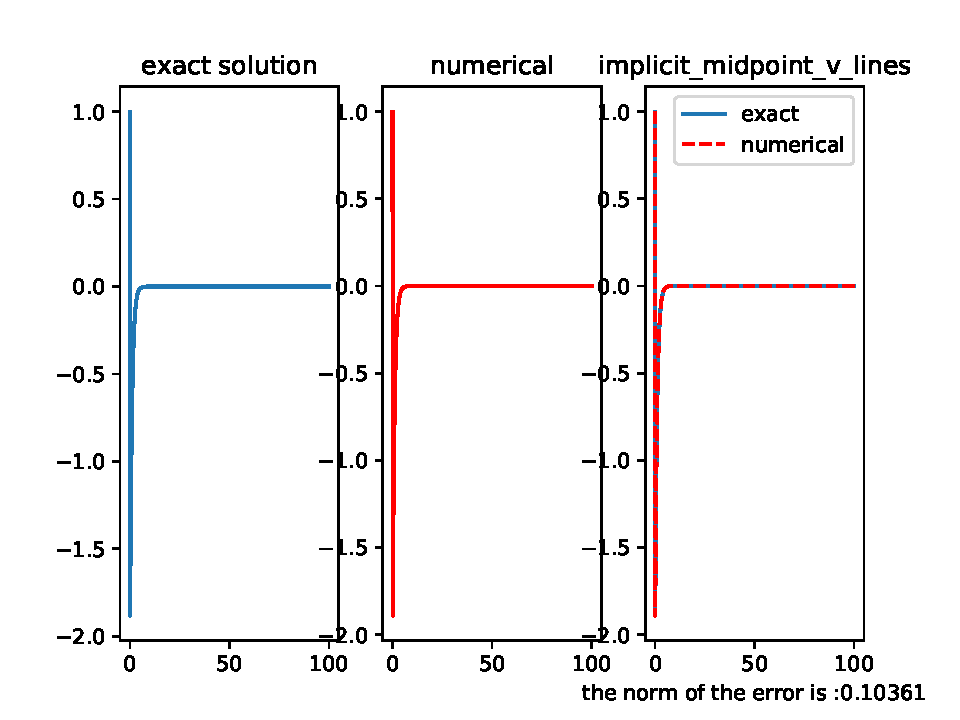
\includegraphics[height=8cm,width=12cm]{implicit_midpoint_v_lines.pdf}
 \end{frame}
 

 \section{Explicit Runge-Kutta Method}
 \begin{frame}{explicit Runge-Kutta Method}
    \[
        \begin{cases}
            u_{n+1} &= u_n +\frac{1}{6}(k_{u1}+2k_{u2}+2k_{u3}+k_{u4})\\
            v_{n+1} &= v_n +\frac{1}{6}(k_{v1}+2k_{v2}+2k_{v3}+k_{v4})
        \end{cases}
        \]
    where 
    \begin{columns}[T] % align columns
        \begin{column}{.48\textwidth}
            \[
                \begin{cases}
                    f_u&=98u+198v\\
                    k_{u1}&=hf_u\\
                    k_{u2}&=h(f_u+\frac{1}{2}k_{u1})\\
                    k_{u3}&=h(f_u+\frac{1}{2}k_{u2})\\
                    k_{u4}&=h(f_u+k_{u3})
                \end{cases}
                \]
    
        \end{column}%
        \hfill%
        \begin{column}{.48\textwidth}
            \[
                \begin{cases}
                    f_v&=-99u-199v\\
                    k_{v1}&=hf_v\\
                    k_{v2}&=h(f_v+\frac{1}{2}k_{v1})\\
                    k_{v3}&=h(f_v+\frac{1}{2}k_{v2})\\
                    k_{v4}&=h(f_v+k_{v3})
                \end{cases}
                \]
        
        \end{column}
    \end{columns}
 \end{frame}
 \begin{frame}{Runge Kutta Result of $u(t)$}

    \centering
    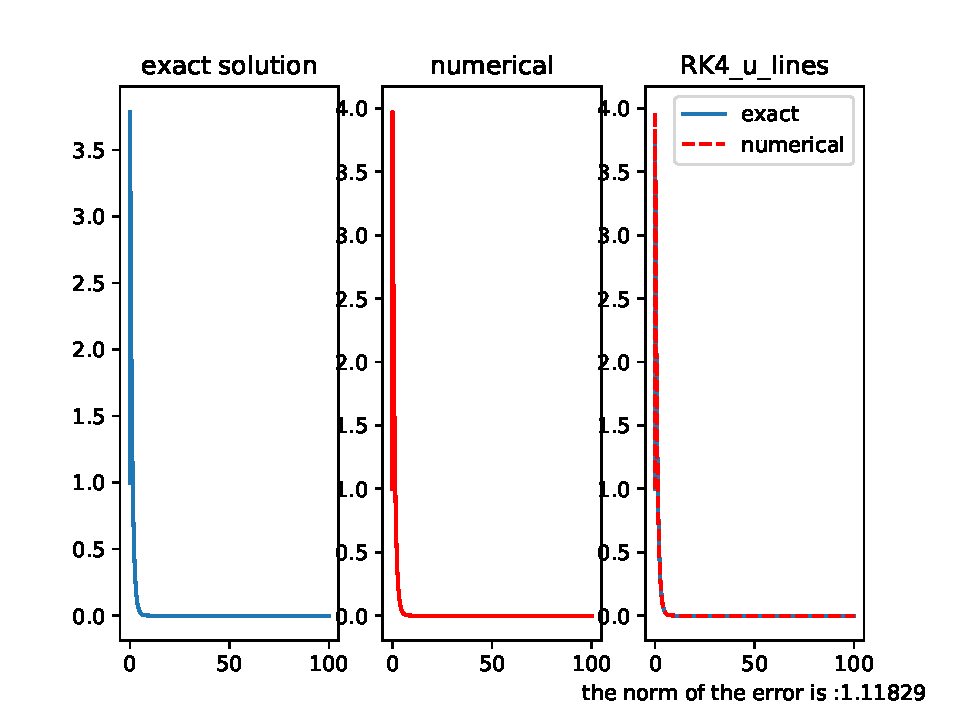
\includegraphics[height=8cm,width=12cm]{RK4_u_lines.pdf}
 \end{frame}
 \begin{frame}{Runge Kutta Result of $v(t)$}
    \centering
    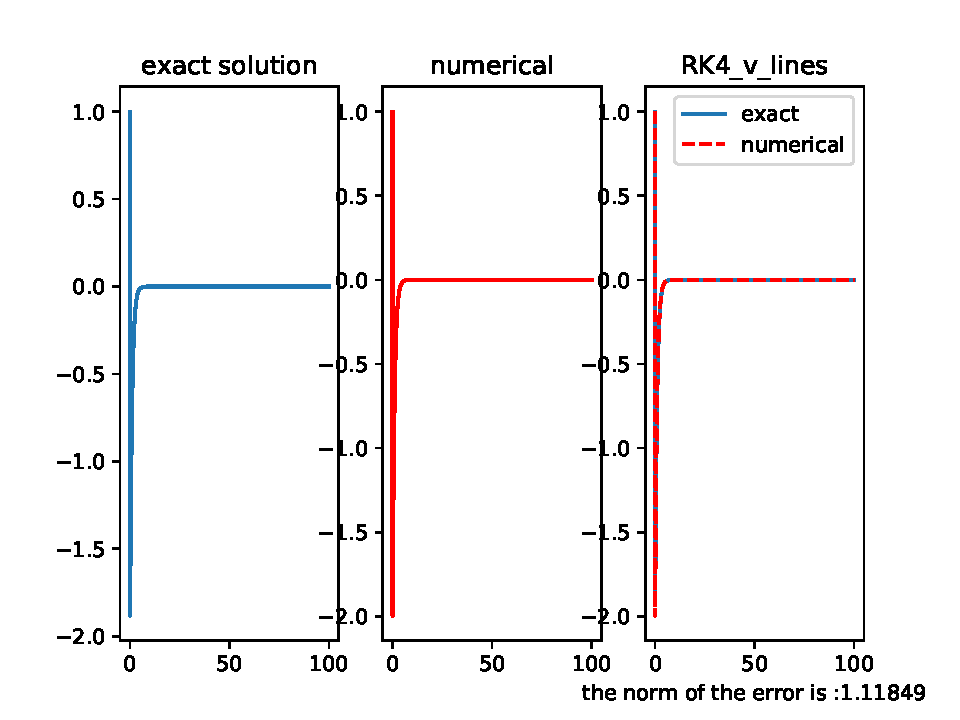
\includegraphics[height=8cm,width=12cm]{RK4_v_lines.pdf}
 \end{frame}
 \begin{frame}[standout]
    Thank you !
 \end{frame}
\end{document}

